\documentclass[11pt]{article}

\usepackage[final]{acl}
\usepackage{times}
\usepackage[T1]{fontenc}
\usepackage[utf8]{inputenc}
\usepackage{microtype}
\usepackage{inconsolata}
\usepackage{graphicx}
\usepackage{xcolor}
\usepackage{tikz}
\usetikzlibrary{arrows.meta,positioning}

\title{Numbers Through Signs:\\
How LLMs Connect Counts, Number Words, and Numerals}

\author{J. Albert Yoo \\
  {\normalsize E\"otv\"os Lor\'and University} \\
  {\small j.albert.yoo.academic@gmail.com}}

\hypersetup{
    pdfauthor={J. Albert Yoo},
    pdftitle={Numbers Through Signs: How LLMs Connect Counts, Number Words, and Numerals},
    pdfsubject={MathNLP 2026 camera-ready paper}}


\begin{document}
\maketitle

\begin{abstract}

Large language models manipulate numerical expressions fluently, yet it is
unclear whether a number inferred from a collection enters the same internal
interface as an explicit numeral or number word. We test digits, English
number words, and counts of repeated tokens in five Qwen3 base models from
0.6B to 14B. After each quantity expression but before a comparison, parity,
or equality question, we interchange one residual-stream state between
forms. Textual-count states preserve held-out cardinal order, even at fixed
sequence length. In behaviourally competent 8B and 14B cases, digit and
number-word states are bidirectionally interchangeable. At the tested
collection boundary, however, a count state does not transfer even to a
different count of the same form, and no count--sign direction meets the
same one-shot criteria. A same-depth sweep and symbol-derived linear subspace
do not recover a bidirectional local interface. Longer interventions and a
separate mixture-of-experts model reveal strong but directional bridges.
Counting information and correct behaviour can therefore coexist without a
locally portable state at the tested boundary.
\end{abstract}

\section{Introduction}


Large language models (LLMs) can manipulate equations, check proof steps, and
answer many mathematical questions, while remaining unexpectedly brittle at
counting repeated items or extracting quantities from ordinary text. Recent
mechanistic work complicates any simple explanation based on missing number
information. Counts can be decoded from language- and vision-language-model
activations, and multi-stage routines can transmit and aggregate counting
signals \citep{hasani2026counting,hasani2026system2}. A model may therefore
contain a count even when its answer is unreliable. The open issue is how that
count participates in the rest of the model's numerical computation.


Related studies find regular geometry across explicit number forms
\citep{stefanik2026universal}, and show that numerical information recoverable
by a probe can exceed what a model expresses in its answers
\citep{yuchi2026numbers}. Low-dimensional, format-agnostic subspaces can also
transfer reasoning more effectively than replacing an entire hidden state
\citep{yuan2026fars}. These results establish numerical structure and usable
signals. They leave a sharper question unanswered: once the model has
constructed the cardinality of a collection, can that state be used in place
of the state produced by a digit or number word in a later operation?


The question matters because human numerical expressions are ordinarily
reused across very different encounters. The mark \emph{3}, the word
\emph{three}, three objects, and three repeated actions can all guide a new
comparison, match, or calculation. Humans develop these abilities through
language embedded in perception, action, and cultural practice. A text-first
LLM follows a strikingly different route: proofs, numerals, descriptions of
objects, and reports of action all reach it through the same stream of signs.
This makes the model an inspectable case for separating fluency with public
mathematical notation from the internal connection between signs and
constructed quantities.


We study that connection with a task-late interchange assay. A Qwen3 model
first reads a quantity as a digit, number word, or enumerated textual
collection. Only after the expression ends does it receive a comparison,
parity, or equality question. We transplant the boundary state from one form
into another and ask whether the model's answer follows the donor number. The
experiments show a robust digit--word interface, but the tested
collection-boundary state is not portable even between two textual counts.
Partial transfer under longer interventions shows that the count--sign
connection is graded rather than absent. For mathematical NLP, the result
separates what behavioural accuracy and numerical probes measure from whether
different expressions feed a common, immediately reusable numerical state.

\section{Task-Late Interchange Assay}

\paragraph{Models, number forms, and tasks.}

We study base Qwen3 checkpoints at 0.6B, 1.7B, 4B, 8B, and 14B parameters
\citep{yang2025qwen3}. Production runs use pinned revisions, BF16 weights and
activations, and one A100 80GB GPU, without quantization or CPU offload. A
Qwen3-30B-A3B checkpoint is analysed separately because sparse expert routing
makes it an architectural contrast rather than a sixth dense scale point.
Cardinalities 2--9 are expressed as an Arabic digit (\texttt{3}), an English
number word (\texttt{three}), a variable-length textual count
(\texttt{[A A A]}), or a shuffled ten-item A/B sequence containing three A
tokens. The last condition keeps total length constant while cardinality
changes. The later questions ask whether the quantity exceeds a threshold,
is odd or even, or equals a threshold.

\begin{figure}[t]
  
  \centering
  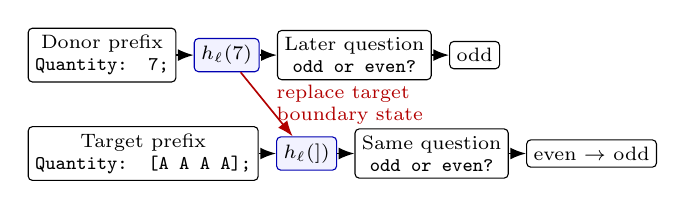
\begin{tikzpicture}[
      x=1cm,y=1cm,
      font=\scriptsize,
      box/.style={draw,rounded corners=1.5pt,inner sep=2.5pt,align=center},
      state/.style={draw=blue!70!black,fill=blue!5,rounded corners=1.5pt,
                    inner sep=2.5pt,align=center},
      answer/.style={draw,rounded corners=1.5pt,inner sep=2.5pt,align=center},
      arrow/.style={-{Latex[length=2mm]},line width=.6pt}
    ]
    \node[box,anchor=west] (donor) at (0,1.25)
      {Donor prefix\\\texttt{Quantity: 7;}};
    \node[state,right=0.22cm of donor] (dstate) {$h_\ell(7)$};
    \node[box,right=0.22cm of dstate] (dquestion)
      {Later question\\\texttt{odd or even?}};
    \node[answer,right=0.22cm of dquestion] (danswer) {odd};
    \node[box,anchor=west] (target) at (0,0)
      {Target prefix\\\texttt{Quantity: [A A A A];}};
    \node[state,right=0.22cm of target] (tstate) {$h_\ell(])$};
    \node[box,right=0.22cm of tstate] (tquestion)
      {Same question\\\texttt{odd or even?}};
    \node[answer,right=0.22cm of tquestion] (tanswer) {even $\rightarrow$ odd};
    \draw[arrow] (donor) -- (dstate);
    \draw[arrow] (dstate) -- (dquestion);
    \draw[arrow] (dquestion) -- (danswer);
    \draw[arrow] (target) -- (tstate);
    \draw[arrow] (tstate) -- (tquestion);
    \draw[arrow] (tquestion) -- (tanswer);
    \draw[arrow,red!70!black] (dstate) -- node[right,align=left]
      {replace target\\boundary state} (tstate);
  \end{tikzpicture}
  \caption{\textbf{One-shot task-late interchange.} The
  donor encodes seven as a digit; the target encodes four as a textual count.
  Both prefixes end before the parity question. If the transplanted state can
  play the donor's numerical role, the target answer changes from even to
  odd. A same-number donor tests whether cross-form replacement preserves the
  original answer.}
  \label{fig:assay}
\end{figure}

\paragraph{Interchange by example.}

Figure~\ref{fig:assay} shows the central intervention. The donor prefix states
seven explicitly; the target prefix presents four repeated tokens. At one
decoder layer, we replace the residual-stream state at the target expression's
closing bracket with the donor state at the digit. The unmodified target
answers \emph{even}; successful counterfactual transfer makes the continuation
follow seven and answer \emph{odd}. Replacing the boundary state with one
derived from a different form of the same number should preserve the target's
answer. Together, counterfactual transfer and same-number preservation test
\emph{local causal interoperability}: whether one task-late state can assume
another form's numerical role in the model's own downstream computation
\citep{geiger2025causal}.

\paragraph{Selection, screening, and measures.}

For each model, the decoder site is selected using development-template
digit--word transfer only; the embedding output is excluded. The selected
sites for the dense series are 3, 4, 6, 6, and 1 in ascending model size.
Evaluation wording is chosen through behaviour alone: digit and word balanced
accuracy must each reach .85, textual-count accuracy .65, each count answer
class must exceed .60, and every principal direction must retain at least 16
trials on which the unmodified donor and target are correct. Conditional
interchange intervention accuracy (IIA) is the proportion of those eligible
trials whose patched answer follows the donor. A same-number donor supplies a
do-no-harm preservation test; exact no-op and wrong-donor trials check the
intervention itself. A direction is counted as established when eligibility
is at least .50, same-number preservation .90, one-shot IIA .80, and the lower
cluster-bootstrap bound on donor-directed logit gain is positive.

\paragraph{Persistence, readouts, and local scope.}

The primary intervention is applied once; additional windows maintain the
donor state over 2, 4, 8, or all remaining decoder sites. For 14B comparison,
we also begin a to-end intervention at every same-depth site. Ridge readouts
leave out one numerical value at a time, and a rank-7 cardinal subspace is
learned only from digit and word development states. The assay targets one
local interface, not an information bottleneck: after the closing-bracket
state is replaced, later tokens can still attend to the original A tokens.

\section{Results}

\begin{figure*}[t]
  \centering
  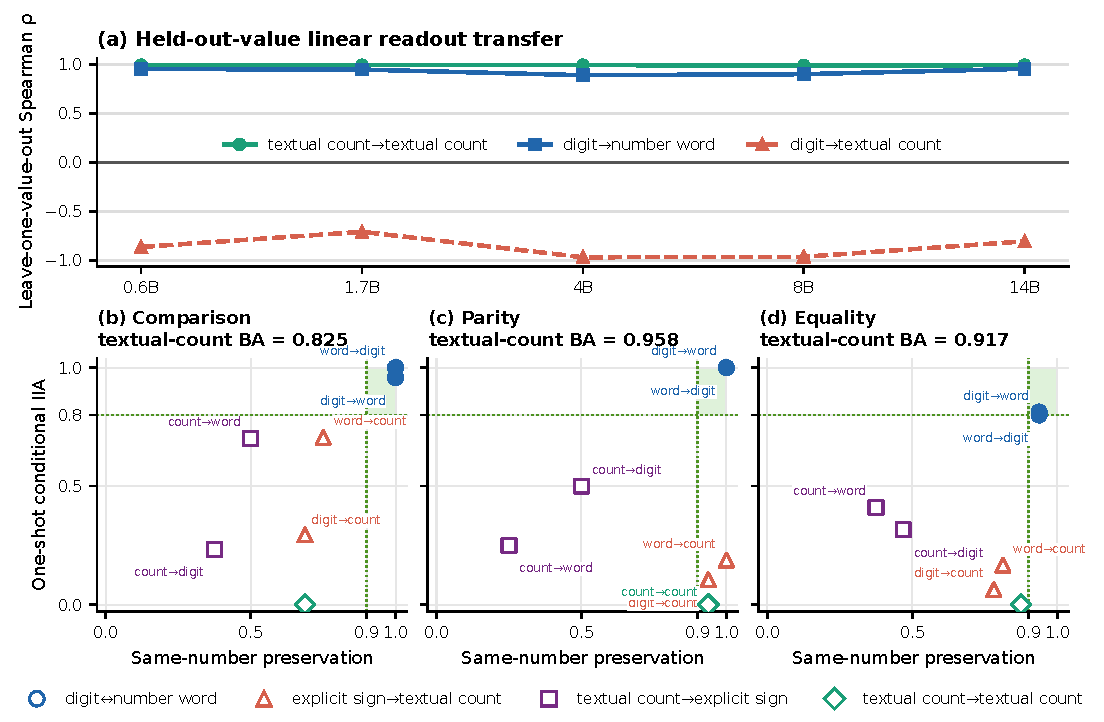
\includegraphics[width=\textwidth]{figure.pdf}
  \caption{\textbf{Cardinal readouts and one-shot interchange.}
  (a) A readout trained on textual counts preserves held-out numerical order;
  a digit-trained readout transfers to number words but not to textual counts.
  The fixed-total control reaches $\rho=.967$--$.993$ within format.
  (b--d) Same-number preservation and conditional IIA for Qwen3-14B on the
  three behaviourally screened tasks, including the previously unreported
  textual-count-to-textual-count baseline. Filled points satisfy the four
  stated one-shot criteria.}
  \label{fig:main}
\end{figure*}

\paragraph{Collection states preserve cardinal order.}

A ridge readout trained on textual-count states orders unseen values with
Spearman $\rho=.990$--$.993$ across all five dense models
(Fig.~\ref{fig:main}a). The fixed-total A/B control reaches
$\rho=.967$--$.993$, so total sequence length is unnecessary for this
within-format result. A digit-trained readout transfers to number words
($\rho=.891$--$.956$). Applied to textual counts, however, the same readout
gives $\rho=-.707$ to $-.967$. The observed rank reversal is directional:
digit-trained readouts also give $\rho=-.775$ to $-.922$ on fixed-total
collections. Varying sequence length therefore does not explain this
systematic misalignment of the tested linear coordinates, whose origin
remains unresolved.

\paragraph{Digits and number words provide the causal anchor.}

Qwen3-14B passes behavioural screening on textual counts for comparison (.825
balanced accuracy), parity (.958), and equality (.917). Across all three
operations, digit and number-word states meet the one-shot criteria in both
directions. Comparison and parity have same-number preservation of 1.000 and
IIA of at least .958 in each direction; equality has preservation of .938 and
IIA of .800--.813. The positive anchor demonstrates that the assay can detect
a locally portable state shared by two expression forms.

\paragraph{Competent counts do not show the same one-shot interface.}

Parity supplies the clearest contrast because every requested 14B
count--sign intervention has correct unmodified endpoints: each direction
contains 48 eligible trials, versus 24 for each explicit-sign direction.
Digit-to-count replacement
preserves a same-number answer at .938 but follows a different donor number
on only .104 of trials; number-word-to-count preservation is 1.000 while IIA
is .188. The two explicit-sign directions score 1.000 on both measures. The
8B model independently passes an equality wording with textual-count
balanced accuracy .813: both digit--word directions meet the criteria, while
none of the four count--sign directions does. Across comparison, parity,
and equality, zero of twelve 14B count--sign directions establish the
one-shot local interface.

\paragraph{The count boundary is not a portable register.}

The full format matrix supplies a same-form baseline. At the selected 14B
site, count-to-count one-shot IIA is zero
for comparison, parity, and equality. Parity is decisive: all 48 trials are
eligible, and preservation is .938 over 16 same-number trials. Thus the tested
closing-bracket state does not carry a counterfactually portable count even
within the collection format; the cross-form null is not merely disagreement
between two portable codes.

\paragraph{Depth and linear-subspace controls preserve the dissociation.}

For 14B comparison, to-end replacement beginning at every same-depth site
finds digit--word transfer at many starting depths, but no identity-valid
bidirectional count--sign relation. A rank-7 subspace learned from digit and
number-word states gives IIA and preservation of 1.000 within the explicit
sign pair. For count-to-digit, subspace replacement raises preservation to
1.000 while IIA remains .067. No count direction becomes bidirectional, nor
do equal-rank random, label-permuted, or top-variance controls reveal one.

\paragraph{Longer interventions reveal partial bridges.}

Count--sign replacements frequently move the output margin towards the
donor even when the categorical answer does not change. Maintaining the
transplanted state can produce much stronger transfer: on 14B parity,
number-word-to-count IIA rises from .188 after one site to .729 over eight.
The separate 30B-A3B mixture-of-experts model provides a stronger boundary
case on one equality wording. Digit-to-count reaches .806 at window 8, and
number-word-to-count reaches .833 at windows 2--8, all with same-number
preservation 1.000. The reverse directions and a second equality wording are
weaker. Text-only training can therefore connect explicit signs to a
constructed count, but the strongest connections remain directional and
dependent on prompt or continued intervention.

\section{Discussion}


The local failures have different immediate diagnostics. Count-to-count and
sign-to-count results show that the closing bracket is not a causal
bottleneck: the model can continue to use the surviving collection tokens,
while sustained sign-to-count intervention increasingly competes with that
evidence. Full-state count-to-sign replacement can also disrupt an
incompatible sign slot. Yet the symbol-subspace count-to-digit intervention
preserves the same-number answer perfectly while transferring the donor on
only .067 of eligible trials. Behavioural numeracy, probe decodability, causal
influence, and immediate cross-format reuse are therefore distinct
measurements for mathematical NLP.


The experiments separate properties often collapsed into saying that a model
``represents'' a number: recoverable information, behavioural use, causal
influence, and immediate reuse across expressions. Broader coordination could
instead be distributed across states and remain flexible across directions,
wordings, and operations. The tested Qwen3 states separate information and
influence from this local form of coordination.


For humans, learning that \emph{3} means \emph{three} is more than memorizing
a pair of marks: both signs can be used for a quantity already encountered in
counting, matching, and acting on collections. Qwen3's digit--word interchange
shows that language training can coordinate signs internally. The
symbol-grounding problem asks how such signs connect beyond one another
\citep{harnad1990symbol}; model tokens may also inherit derivative reference
from the human practices recorded in their data \citep{mandelkern2024refer}.
Our dissociation concerns how far that inherited practice organises the
model's own collection-derived states.


Embodied accounts suggest why human numerical uses may integrate readily
\citep{lakoff2000where,winter2020metaphor}. The body need not store an
abstract object called three. It can provide a common causal ground: matching,
repetition, distribution, addition, removal, and persistence constrain signs
and situations through recurring successes and failures. The familiar
\emph{felt threeness} of three objects or actions marks a phenomenological
contrast; our experiment tests functional organisation, not experience.
Infants distinguish small-set tracking from approximate magnitude systems
\citep{feigenson2004core}, while non-human animals act selectively on quantity
with limited public symbolism \citep{nieder2021neuroethology}. Text-first LLMs
expose the complementary case: extensive public symbolism without a history
of quantity-guided action. How nonsymbolic quantity connects to exact number
words remains disputed \citep{leibovich2016symbol}.


The positive results sharpen this contrast. Qwen3-14B coordinates explicit
signs tightly, while the MoE model develops strong symbol-to-count transfer
under sustained intervention. Such directional, unstable bridges differ from
flexible reuse across human numerical practice. Testing embodied development
requires changing how numerical forms are learned, not further interpreting
one pretrained text-only family.

\section{Conclusion}


Textual counts carry cardinal information and enter partial causal bridges,
but do not share the portable digit--word interface. At the tested boundary
in competent 8B and 14B models, a count state transfers neither within its
format nor to an explicit sign after one shot. Same-depth and symbol-subspace
tests do not restore bidirectional transfer; longer interventions reveal a
fragile connection.

\clearpage
\section*{Limitations}


The five dense checkpoints belong to one model family and do not provide a
controlled scaling law. Cardinalities are restricted to 2--9, and every
collection is textual. Three comparison, three parity, and four equality
wordings were screened; one 14B wording per operation passed the behaviour-only
rule. The principal causal results therefore concern prompts with adequate
baseline competence rather than prompt variation in general.
The cluster-bootstrap intervals summarise variation over eight source values
within this finite synthetic design; they do not estimate a population over
numbers, prompts, model families, or independently trained checkpoints. The
30B-A3B contrast changes sparse routing, total parameter count, active
parameter count, and other properties together.


The intervention replaces one task-late token. The original items in a
textual collection remain available through attention, allowing a
counterfactual donor state to compete with surviving target evidence. Source
and target states are compared only at the same decoder depth. The experiments
therefore leave open distributed, multi-token, nonlinear, temporally shifted,
and collection-trained interfaces. The all-depth sweep covers same-depth
correspondences, while ridge readouts and the rank-7 symbol-derived subspace
test linear coordinates learned from specific development templates.


The operations and thresholds measure local causal interoperability rather
than grounding, phenomenal experience, or a complete theory of mathematical
understanding. No model learned quantity through perception or action. A
direct follow-up could train matched agents in a synthetic 2-D environment
under three curricula: text-only descriptions, passive views of collections,
and action-contingent tasks requiring agents to match, produce, and distribute
$n$ objects. Novel signs could be learned in disjoint contexts without direct
pairing. Their later bidirectional reuse across new prompts and operations
would test whether shared success conditions create the common numerical
ground proposed here.

\section*{Acknowledgements}


Generative AI tools assisted with literature search, coding, experiment
orchestration, language editing of author-supplied material, and low-novelty
drafting of factual Methods and Results descriptions from verified records.
The substantive research questions, philosophical claims, and interpretations
were supplied by the human author. Final verification, approval of every
sentence, and responsibility for the submitted work remain with the human
author. AI systems are not authors.

\bibliography{references}

\end{document}
